% Boundary conditions of the DNS problem (Eq. bc) and of the homogenized problem (Eq. macro_problem).
% Compile: pdflatex bc_dns.tex  ->  bc_dns.pdf  (copied to ../bc_dns.pdf)
\documentclass[tikz,border=3pt]{standalone}
\usepackage{amsmath,amssymb}
\usetikzlibrary{arrows.meta}
% Shared colours and line styles of the boundary-condition diagrams.
\definecolor{dir}{HTML}{B03A2E}       % Dirichlet (imposed temperature)
\definecolor{neu}{HTML}{1F4E79}       % Neumann (insulated)
\definecolor{per}{HTML}{1E8449}       % periodic
\definecolor{solidfill}{HTML}{E9EEF3} % solid material
\definecolor{homfill}{HTML}{D6E4F0}   % homogenized material
\definecolor{layer}{HTML}{F0B27A}     % boundary layer
\tikzset{insul/.style={densely dashed}}

\begin{document}
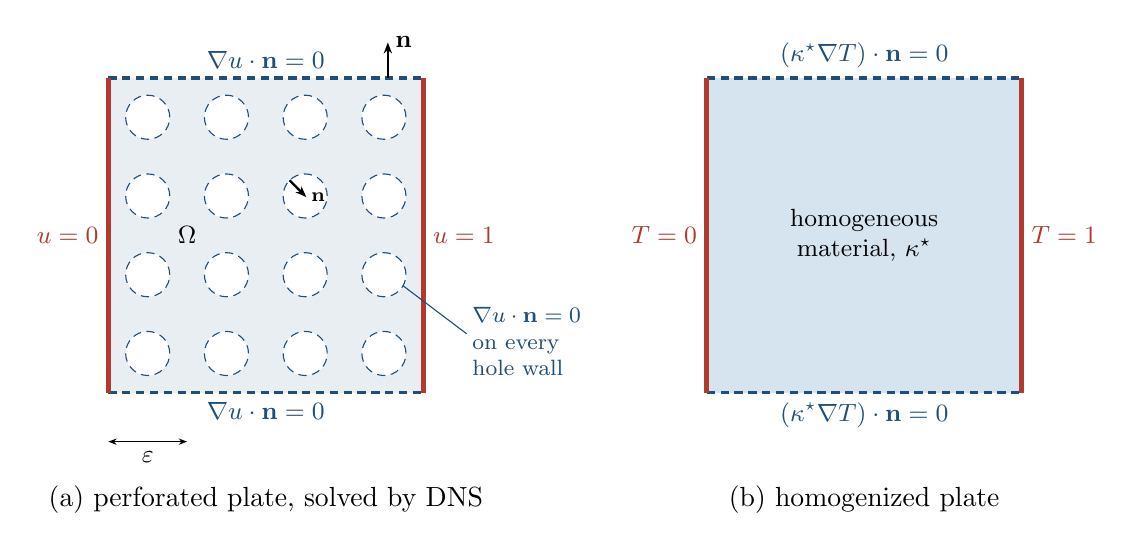
\begin{tikzpicture}[font=\small]
  % ---------------- (a) perforated plate ----------------
  \begin{scope}
    \fill[solidfill] (0,0) rectangle (4,4);
    \foreach \i in {0,...,3}{\foreach \j in {0,...,3}{
      \fill[white] (\i+0.5,\j+0.5) circle (0.28);
      \draw[neu, insul] (\i+0.5,\j+0.5) circle (0.28);}}
    \draw[neu, insul, very thick] (0,0) -- (4,0);
    \draw[neu, insul, very thick] (0,4) -- (4,4);
    \draw[dir, line width=1.8pt] (0,0) -- (0,4);
    \draw[dir, line width=1.8pt] (4,0) -- (4,4);
    \node[dir, left]  at (0,2) {$u=0$};
    \node[dir, right] at (4,2) {$u=1$};
    \node[neu, above] at (2,4) {$\nabla u\cdot\mathbf{n}=0$};
    \node[neu, below] at (2,0) {$\nabla u\cdot\mathbf{n}=0$};
    % outward normals
    \draw[-{Stealth[length=4pt]}, thick] (3.55,4) -- (3.55,4.45) node[right=-1pt] {$\mathbf{n}$};
    \draw[-{Stealth[length=4pt]}, thick] ({2.5+0.28*cos(135)},{2.5+0.28*sin(135)}) -- ++(-45:0.3)
         node[right=-2pt, font=\scriptsize] {$\mathbf{n}$};
    % hole callout
    \draw[neu, thin] ({3.5+0.28*cos(-30)},{1.5+0.28*sin(-30)}) -- (4.55,0.75);
    \node[neu, right, align=left, font=\footnotesize] at (4.5,0.65) {$\nabla u\cdot\mathbf{n}=0$\\on every\\hole wall};
    \node at (1.0,2.0) [fill=solidfill, inner sep=1pt] {$\Omega$};
    % cell size
    \draw[{Stealth[length=3pt]}-{Stealth[length=3pt]}] (0,-0.62) -- (1,-0.62) node[midway, below] {$\varepsilon$};
    \node[font=\normalsize] at (2,-1.35) {(a) perforated plate, solved by DNS};
  \end{scope}
  % ---------------- (b) homogenized plate ----------------
  \begin{scope}[xshift=7.6cm]
    \fill[homfill] (0,0) rectangle (4,4);
    \draw[neu, insul, very thick] (0,0) -- (4,0);
    \draw[neu, insul, very thick] (0,4) -- (4,4);
    \draw[dir, line width=1.8pt] (0,0) -- (0,4);
    \draw[dir, line width=1.8pt] (4,0) -- (4,4);
    \node[dir, left]  at (0,2) {$T=0$};
    \node[dir, right] at (4,2) {$T=1$};
    \node[neu, above] at (2,4) {$(\kappa^{\star}\nabla T)\cdot\mathbf{n}=0$};
    \node[neu, below] at (2,0) {$(\kappa^{\star}\nabla T)\cdot\mathbf{n}=0$};
    \node[align=center] at (2,2) {homogeneous\\material, $\kappa^{\star}$};
    \node[font=\normalsize] at (2,-1.35) {(b) homogenized plate};
  \end{scope}
\end{tikzpicture}
\end{document}
